
\chapter{Project Context}
\begin{spacing}{1.3}

\section{Clinical Background}

Melanoma ranks as the most lethal form of skin cancer, responsible for the overwhelming majority of skin cancer fatalities worldwide. According to the American Cancer Society, approximately 100,000 new cases of invasive melanoma are diagnosed annually in the United States alone, with over 8,000 deaths attributed to the disease each year. Global incidence has risen steadily over the past three decades, with particularly sharp increases in fair-skinned populations exposed to high levels of ultraviolet radiation.

The prognosis for melanoma patients is dramatically stage-dependent. Early-stage detection (Stage~I) yields a 5-year survival rate exceeding 99\%, as the malignancy remains confined to the epidermis and is curable through simple excision. In contrast, late-stage detection (Stage~IV), where the cancer has metastasised to distant organs, carries a 5-year survival rate below 30\%. This 70-percentage-point gulf in outcomes constitutes one of the strongest clinical imperatives in oncology: early detection saves lives.

Dermoscopy -- the use of a handheld polarised-light magnifier to visualise subsurface skin structures -- improves diagnostic accuracy by 30--50\% over naked-eye examination. However, dermoscopic interpretation requires substantial training. Expert dermatologists achieve sensitivity of approximately 90\% and specificity of approximately 85\%, but general practitioners and non-specialists perform significantly worse. The World Health Organization reports a global shortage of dermatologists, with the most acute deficits in low- and middle-income countries.

Automated melanoma screening systems deployed on edge devices offer a compelling solution to these access barriers. An edge device -- such as a smartphone, tablet, or Raspberry Pi -- can run inference locally without requiring an internet connection. This confers several critical advantages: offline operation in remote clinics, no cloud dependency preserving patient data privacy, instant results with 20--200 millisecond inference latency, and low cost making the technology accessible in resource-constrained settings.

This project is a research and educational prototype. It is not a medical device and has not been evaluated by any regulatory authority. All predictions are for informational purposes only. The pipeline is designed with safety guardrails -- uncertainty quantification, confidence thresholds, and mandatory clinical review flags -- that align with regulatory best practices, but it has not undergone the clinical validation required for real-world deployment.

\section{The HAM10000 Dataset}

The Human Against Machine 10000 (HAM10000) dataset, published by Tschandl et al.~\cite{tschandl2018}, is the largest publicly available collection of dermoscopic images. It contains 10,015 dermatoscopic images acquired at the Department of Dermatology, Medical University of Vienna, Austria, spanning seven diagnostic categories.

\begin{figure}[H]
\centering
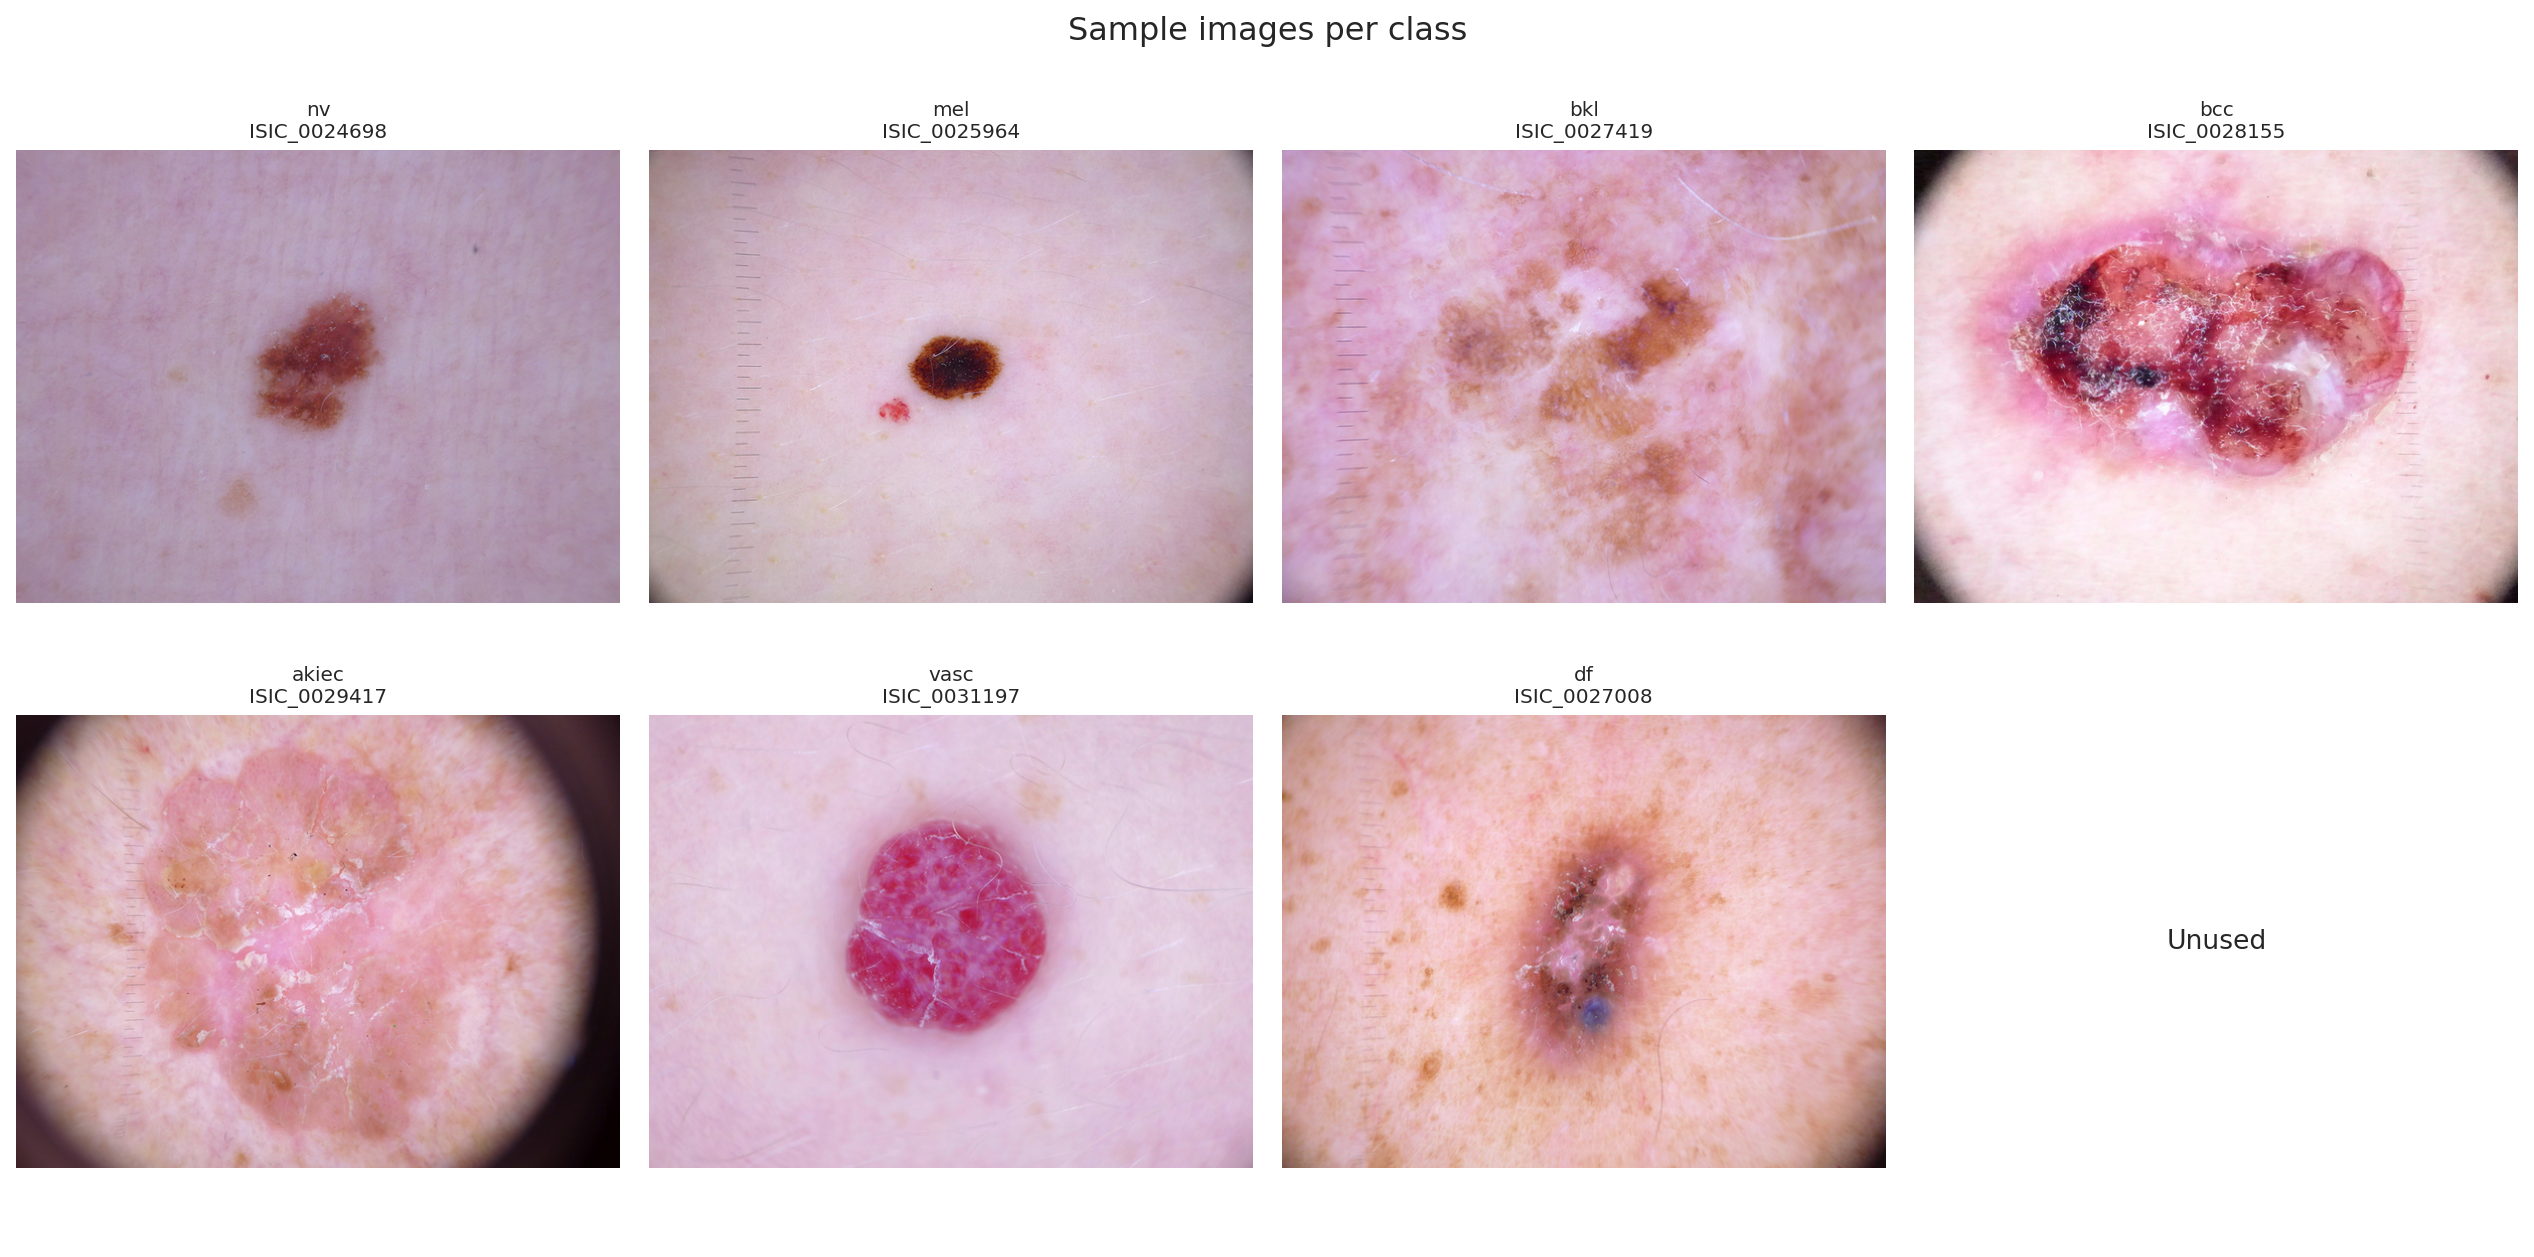
\includegraphics[width=0.65\textwidth]{../figures/ham10000_sample_images.png}
\caption{Sample images from the HAM10000 dataset across seven diagnostic categories.}
\label{fig:ham_samples}
\end{figure}

The dataset presents significant class imbalance, as shown in Table~\ref{tab:ham_dist} and Figure~\ref{fig:class_dist}. Melanocytic nevi dominate at 6,705 samples (66.9\%), while melanoma -- the class of greatest clinical interest -- constitutes only 1,113 samples (11.1\%). For this project, all classes are collapsed into a binary classification task: \textit{benign} (nv, bkl, vasc, df; 8,061 images) and \textit{melanoma} (mel, bcc, akiec; 1,954 images), yielding an 8:1 benign-to-melanoma ratio.

\begin{table}[H]
\centering
\caption{Class distribution of the HAM10000 dataset.}
\label{tab:ham_dist}
\begin{tabular}{lrr}
\toprule
\textbf{Diagnostic Category} & \textbf{Abbreviation} & \textbf{Count} \\
\midrule
Melanocytic nevi          & nv  & 6,705 \\
Melanoma                  & mel & 1,113 \\
Benign keratosis-like lesions & bkl & 1,099 \\
Basal cell carcinoma      & bcc & 514  \\
Actinic keratoses         & akiec & 327 \\
Vascular lesions          & vasc & 142  \\
Dermatofibroma            & df  & 115  \\
\midrule
\textbf{Total}            &     & \textbf{10,015} \\
\bottomrule
\end{tabular}
\end{table}

\begin{figure}[H]
\centering
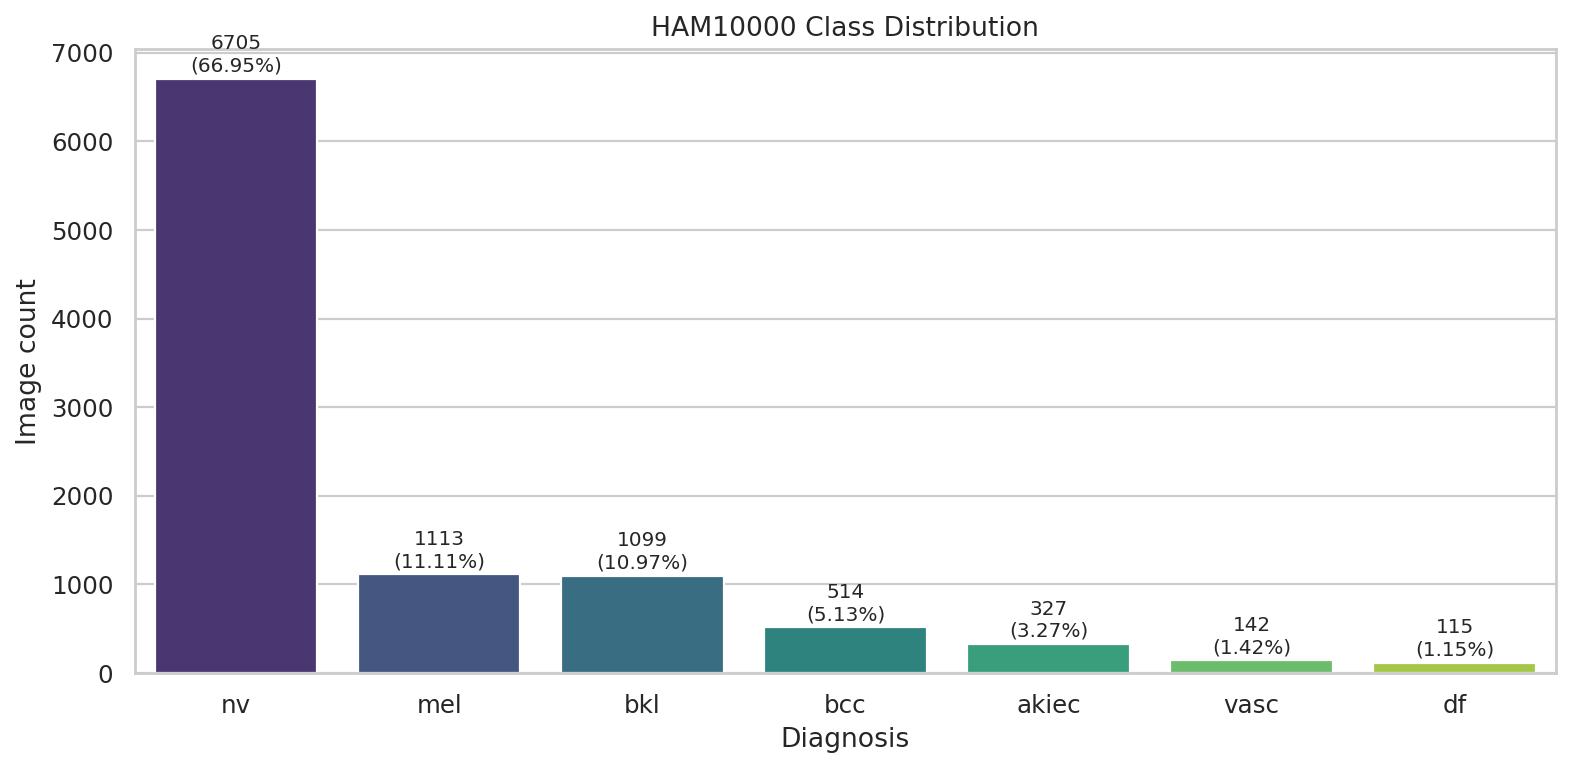
\includegraphics[width=0.6\textwidth]{../figures/ham10000_class_distribution.png}
\caption{Class distribution of HAM10000.}
\label{fig:class_dist}
\end{figure}

\section{Patient-Aware Data Splitting}

Patient-aware splitting is a critical requirement in medical imaging. The HAM10000 dataset contains 7,466 unique lesions, each identified by a lesion identifier. Multiple images may depict the same lesion from different angles or with different imaging modalities. If images from the same lesion appear in both training and test sets, the model can memorise lesion-specific visual signatures rather than learning disease-level features, inflating performance metrics by 5--15 AUC points.

The GroupShuffleSplit strategy with groups set to the lesion identifier allocates 70\% of images to training (6,959 images), 15\% to validation (1,529 images), and 15\% to testing (1,527 images) with a fixed random seed of 42. A two-stage split is performed: first, a 70/30 train/temporary split; then the 30\% temporary split is halved into validation and test.

Zero-leakage verification is performed by set-intersection assertion: the intersection of lesion identifiers between any pair of splits (train/val, train/test, val/test) must be empty. All three assertions passed, confirming 100\% isolation of patient-level data across splits. This satisfies the non-negotiable requirement of zero patient data leakage.

\begin{figure}[H]
\centering
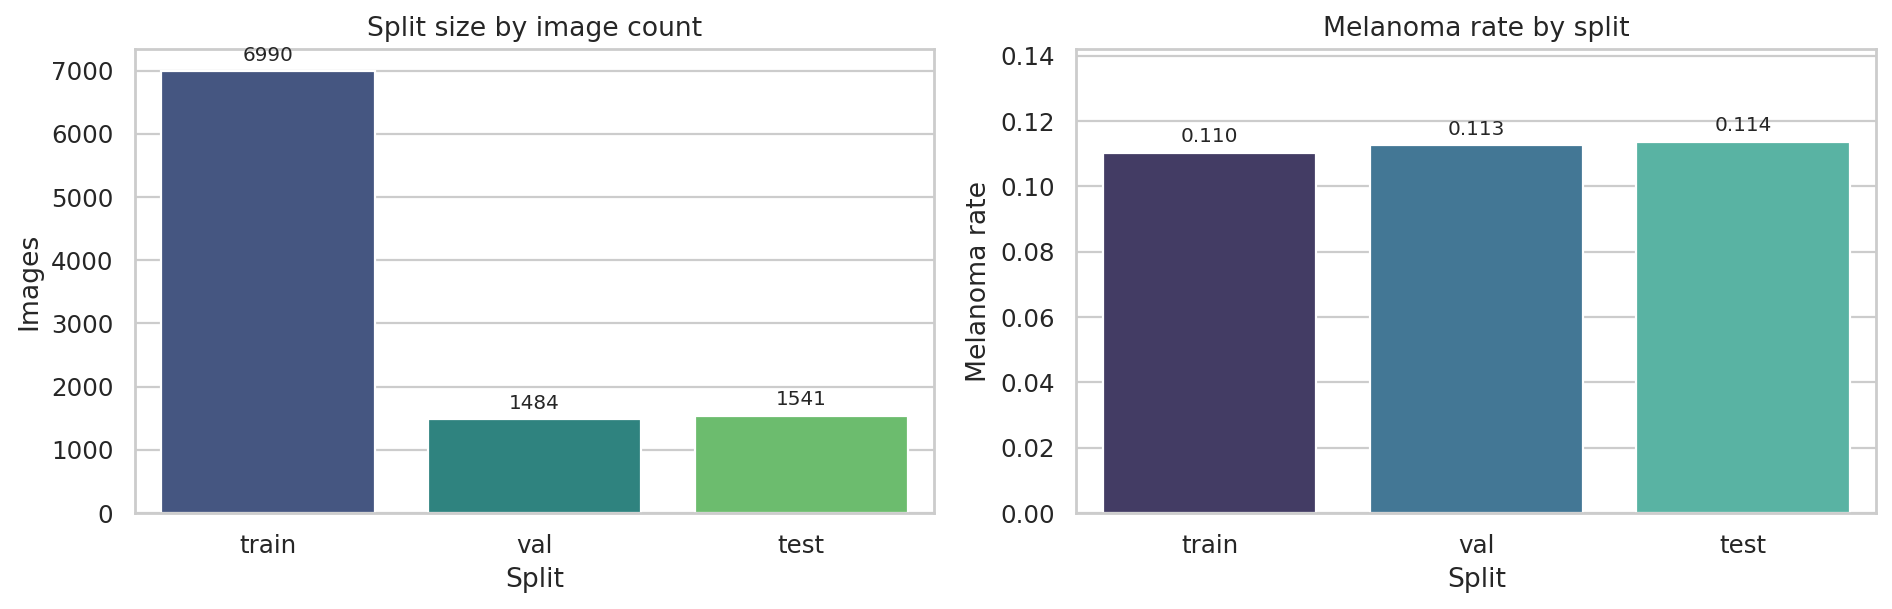
\includegraphics[width=0.6\textwidth]{../figures/ham10000_split_summary.png}
\caption{Train/validation/test split distribution.}
\label{fig:split_summary}
\end{figure}

\section{MLOps Pipeline Architecture}

The core contribution of this project is a complete, end-to-end MLOps pipeline that transforms raw dermoscopic images into a production-ready, edge-deployable melanoma detection API. The pipeline follows a linear progression through 12 distinct phases, illustrated in Figure~\ref{fig:pipeline}.

\begin{figure}[H]
\centering
\begin{tikzpicture}[
    node distance=0.4cm and 0.15cm,
    phase/.style={rectangle, rounded corners=3pt, draw=black!60, fill=blue!8, text width=1.15cm, align=center, minimum height=0.85cm, font=\scriptsize},
    arrow/.style={-{Stealth[length=3pt]}, thick, black!50},
]
% Row 1: Phases 0-5
\node[phase] (p0) {Phase 0\\Env.\\Bootstrap};
\node[phase, right=of p0] (p1) {Phase 1\\Data\\Layer};
\node[phase, right=of p1] (p2) {Phase 2\\Validation};
\node[phase, right=of p2] (p3) {Phase 3\\Preprocess};
\node[phase, right=of p3] (p4) {Phase 4\\Training};
\node[phase, right=of p4] (p5) {Phase 5\\Explain.};

% Row 2: Phases 6-11
\node[phase, below=0.7cm of p0] (p6) {Phase 6\\Optimiz.};
\node[phase, right=of p6] (p7) {Phase 7\\Inference\\API};
\node[phase, right=of p7] (p8) {Phase 8\\Deploy.};
\node[phase, right=of p8] (p9) {Phase 9\\Monitor.};
\node[phase, right=of p9] (p10) {Ph. 10--11\\CI/CD};

% Row 1 arrows
\draw[arrow] (p0) -- (p1);
\draw[arrow] (p1) -- (p2);
\draw[arrow] (p2) -- (p3);
\draw[arrow] (p3) -- (p4);
\draw[arrow] (p4) -- (p5);

% Row transition (p5 to p6) -- curved arrow underneath
\draw[arrow, rounded corners=4pt] (p5.south) -- ++(0,-0.5) -| (p0.south) -- ++(0,-0.2) -| (p6.north);

% Row 2 arrows
\draw[arrow] (p6) -- (p7);
\draw[arrow] (p7) -- (p8);
\draw[arrow] (p8) -- (p9);
\draw[arrow] (p9) -- (p10);
\end{tikzpicture}
\caption{MLOps pipeline: 12-phase progression from environment setup to CI/CD.}
\label{fig:pipeline}
\end{figure}

Phase~0 (Environment Bootstrap) establishes dependency management with uv and pyproject.toml, pre-commit hooks, and DVC initialisation. Phase~1 (Data Layer) handles HAM10000 ingestion and patient-aware stratified splitting. Phase~2 (Data Validation) runs a Great Expectations suite with 7 expectations, 100\% image integrity verification, and duplicate detection. Phase~3 (Preprocessing) applies DullRazor hair removal, Macenko colour normalisation, Albumentations augmentation, and class balancing. Phase~4 (Model Training) trains three architectures with two-phase strategy and full MLflow tracking. Phase~5 (Explainability) implements Grad-CAM, MC-Dropout uncertainty, and temperature scaling calibration. Phase~6 (Model Optimization) handles ONNX export, INT8 quantisation, and latency benchmarking. Phase~7 (Inference API) deploys a FastAPI application with 6 endpoints and safety guardrails. Phase~8 (Deployment) uses multi-stage Docker builds for x86 and ARM64 targets. Phase~9 (Monitoring) instruments Prometheus metrics, structlog logging, and Evidently AI drift detection. Phases~10--11 integrate reliability engineering and GitHub Actions CI/CD.

DVC orchestrates a 6-stage pipeline defined in dvc.yaml, with each stage declaring its dependencies and outputs, enabling deterministic reproduction: \texttt{split\_data} produces patient-aware splits, \texttt{validate\_data} generates GE checkpoints, \texttt{preprocess} produces normalised and augmented images, \texttt{train} generates PyTorch checkpoints and MLflow runs, \texttt{export\_onnx} converts to ONNX format, and \texttt{quantize} produces INT8 optimised models.

\section{Model Architectures}

Three convolutional neural network architectures were evaluated. The primary selection criterion was the accuracy--efficiency frontier: the model must achieve clinically useful discrimination while fitting within the computational budget of a Raspberry Pi~4 (1~GB RAM, ARM Cortex-A72).

EfficientNet-B0~\cite{tan2019} is the baseline member of the EfficientNet family, which introduced compound scaling -- simultaneously scaling depth, width, and resolution using a principled coefficient. With 4.3 million parameters, it achieves state-of-the-art accuracy on ImageNet while being an order of magnitude smaller than conventional architectures, making it the selected production model.

ResNet50 serves as a well-established baseline with 24 million parameters. Its residual connections mitigate the vanishing gradient problem, enabling deeper networks. MobileNetV3-Small~\cite{howard2019} represents the ultra-low-resource extreme at only 1.5 million parameters, serving as a fallback for devices with extremely limited memory.

All three models share a common classifier head architecture:

\[
\begin{aligned}
\text{GlobalAvgPool} \rightarrow \text{BatchNorm1d} \rightarrow \text{Dropout}(p=0.3) \rightarrow \text{Linear}(F,~256) \\
\rightarrow \text{ReLU} \rightarrow \text{Dropout}(p=0.2) \rightarrow \text{Linear}(256,~2)
\end{aligned}
\]

where \(F\) is the backbone-specific feature dimension: 1280 for EfficientNet-B0, 2048 for ResNet50, and 576 for MobileNetV3-Small.

Training proceeds in two phases. Phase~1 (frozen backbone, 10 epochs) trains only the classifier head with learning rate \(1 \times 10^{-3}\) and cosine annealing. Phase~2 (full fine-tuning, 30 epochs) unfreezes all parameters with differential learning rates -- \(1 \times 10^{-4}\) for the backbone and \(1 \times 10^{-3}\) for the head -- plus gradient clipping at \(\text{max\_norm}=1.0\) and early stopping with patience of 8 epochs. Focal Loss~\cite{lin2017} with \(\gamma = 2.0\) and effective-number class weights addresses the 8:1 class imbalance.

\section{Tooling Stack}

The pipeline integrates 13 open-source tools, each selected for a specific role in the MLOps lifecycle. Selection criteria included open-source licensing, active community maintenance, Python 3.10 compatibility, and ARM64/Linux support for the edge deployment target.

\begin{table}[H]
\centering
\caption{MLOps technology stack.}
\label{tab:stack}
\begin{tabular}{lll}
\toprule
\textbf{Category} & \textbf{Tool} & \textbf{Purpose} \\
\midrule
Package Management & uv + pyproject.toml & Dependency management \\
Data Versioning & DVC & 6-stage reproducible pipeline \\
Data Validation & Great Expectations & 7-expectation suite, HTML reports \\
Experiment Tracking & MLflow & Run tracking, params, artifacts \\
Model Format & ONNX & Hardware-agnostic inference \\
Inference Engine & ONNX Runtime & CPU-optimised, INT8 support \\
API Framework & FastAPI & Async REST, auto-docs \\
Containerisation & Docker & Multi-stage, x86 + ARM64 \\
CI/CD & GitHub Actions & Lint, test, build, security scan \\
Monitoring & Prometheus + Evidently & Metrics + drift detection \\
Logging & structlog & Structured JSON logging \\
Frontend & Gradio + HF Spaces & Interactive public demo \\
Task Runner & Makefile + dvc.yaml & Build, test, deploy automation \\
\bottomrule
\end{tabular}
\end{table}

\end{spacing}
